%%%%%%%%%%%%%%%%%%%%%%%%%%%%%%%%%%%%%%%%%%%%%%%%%%%%%%%%%%%%%%%%%%%%%%%%%%%%%%%%
%2345678901234567890123456789012345678901234567890123456789012345678901234567890
%        1         2         3         4         5         6         7         8

\documentclass[letterpaper, 10 pt, conference]{ieeeconf}  % Comment this line out if you need a4paper

%\documentclass[a4paper, 10pt, conference]{ieeeconf}      % Use this line for a4 paper

\IEEEoverridecommandlockouts                              % This command is only needed if 
                                                          % you want to use the \thanks command

\overrideIEEEmargins                                      % Needed to meet printer requirements.

% See the \addtolength command later in the file to balance the column lengths
% on the last page of the document

% The following packages can be found on http:\\www.ctan.org
%\usepackage{graphics} % for pdf, bitmapped graphics files
%\usepackage{epsfig} % for postscript graphics files
%\usepackage{mathptmx} % assumes new font selection scheme installed
%\usepackage{times} % assumes new font selection scheme installed
%\usepackage{amsmath} % assumes amsmath package installed
%\usepackage{amssymb}  % assumes amsmath package installed

\usepackage{graphicx}
\usepackage{amsmath} 
\usepackage{amssymb}
\usepackage{multirow}
\usepackage{subfigure}

\def\degree{${}^{\circ}$}
	  
\title{\LARGE \bf
Robot Path Planning Using Newton-Raphson method Based on RRT-GD
}


\author{Junxiang Ge, Fuchun Sun, Chunfang Liu$^{1}$% <-this % stops a space
%\thanks{*This work was not supported by any organization}% <-this % stops a space
\thanks{$^{1}$State Key Lab of Intelligent Technology and Systems, Tsinghua National Laboratory for Information Science and Technology (TNList), Department of Computer Science and Technology, Tsinghua University.
        {\tt\small gejx14@mails.tsinghua.edu.cn, fcsun@tsinghua.edu.cn}}%
}

\begin{document}



\maketitle
\thispagestyle{empty}
\pagestyle{empty}


%%%%%%%%%%%%%%%%%%%%%%%%%%%%%%%%%%%%%%%%%%%%%%%%%%%%%%%%%%%%%%%%%%%%%%%%%%%%%%%%
\begin{abstract}

We proposed a new method on 7-arm redundant manipulator for obstacle-avoiding path planning. As we all know, RRT (rapidly-exploring random tree) algorithm performs well when doing obstacle-avoiding works, but sometimes it is not fast enough and less goal-direction. In this paper, we use RRT method in the configuration space(C-space), concentrating on both the end actuator’s status and the joints’ movements. In order to reduce the time for path planning, i.e., reduce the steps when doing RRT, we change RRT algorithm to be goal-directionality (we call it RRT-GD), to be adapted to our common works. With this improve, we can see in this paper that result could be reached in less than 10 steps usually, while the original RRT algorithm needs often more than 100 steps doing the same task, i.e., RRT-GD tends to be 10 or more times faster than the usual RRT algorithm. In addition, we apply Newton-Raphson method to do inverse kinematics optimization, thus we can focus on both the status space(S-space) and C-Space. In the end, we use quintic polynomial to smooth the planning path.

\end{abstract}


%%%%%%%%%%%%%%%%%%%%%%%%%%%%%%%%%%%%%%%%%%%%%%%%%%%%%%%%%%%%%%%%%%%%%%%%%%%%%%%%
\section{Introduction}

As we all know, RRT (Rapidly-exploring random tree) is rapidly used in obstacle-avoiding path planning for redundant manipulator. It constructs a graph of obstacle free points in feasible space based on random sampling, in which we search the feasible path from the initial point to goal point. As a result of this, there are some great properties with RRT method compared to other obstacle-avoiding method:
\begin{itemize}
\item RRT method attends to explore unknown space. 
\item The graph constructed by RRT will gradually fill up the feasible space if the exploring times is enough.
\item RRT method don't need precise modeling of the obstacles, instead, it only needs the information if or not a point is obstacle free through doing collision detect, thus ending up with the high efficiency of obstacle free planning.
\end{itemize}

Though it has these advantages, RRT will still perform low planning success rate when there is many obstacles surrounded, or the distance from initial point to goal point is far. In this way, Kuffner proposed a bidirectional RRT algorithm, called bi-RRT, also called RRT-connect, to solve this problem. Within this method, two trees were built based on the initial point and goal point separately. When expanding each time, the tree of initial point will extend to the goal-point based tree, or the contrary way, until these two trees meets. Cause it has goal heuristic, it improves the success rate of path planning.  

In spite of these advantages of RRT and its modified algorithm, we still find it defective sometimes in doing our common works. As mentioned before, RRT attends to explore unknown space, so that it could exploring the whole free space. But we just don’t need to explore the whole space the most time when doing simply goal-reaching works. In this way, all we need to do is to find a feasible way from initial point to goal point without obstacle collision, i.e., we only need to explore a part of the whole space including initial point, goal point, and some obstacles. Thus we proposed RRT-GD (RRT with goal-directionality), using the train of thought above. As we can see later in this paper, by doing this way, we can get the result rapidly, usually ten times faster than the normal RRT method.

As we doing RRT in C-space (configuration space), we need to compute the joint angles of each point in the path tree, i.e., inverse kinematics optimization. There are also a lot of methods to do inverse kinematics optimization, e.g., GP (gradient projection method), WLN (weighted least norm	 method), extended Jacobi method, etc. In this paper, we adopt Newton-Raphson method to do this inverse kinematics optimization work. Compared to other methods, Newton-Raphson method performs faster and more accurate. Provided the result can get by Newton-Raphson method, it would take less than 10 iteration times (usually 5 or 6 times), with bias less than micro-meters. 

After we get the path from initial point to goal point, with detailed status information (pose \& joint angles), we then use quintic polynomial to smooth the path [9]. 

We organize this paper according to our experiment process, to show our results more fluently. First, we discuss the basic mathematics knowledge and algorithm we use, including RRT and its modified method in more detail. Then, we introduce Newton-Raphson method in inverse kinematics by using the normal RRT method. After that, we present quintic polynomial method in smoothing path. Later, in order to accelerate the path planning process and doing works in real-time, we propose RRT-GD method, which press more close to our tasks in common use.

\section{Experiment Environment}

All the results we show is based on a redundant robot arm. Before introduce our algorithm, we can have a look at the basic environment.

\subsection{Robot Model \& Its Relevant Variables}

We use a 7-arm redundant robot manipulator to test the results in our experiment. We use the DH method (Denavit and Hartenberg method) to model our robot arm, with the model axis built obeying D-H parameter method as the Fig. 1 show.

   \begin{figure}[thpb]
      \centering
      \framebox{\parbox{2.2in}
      {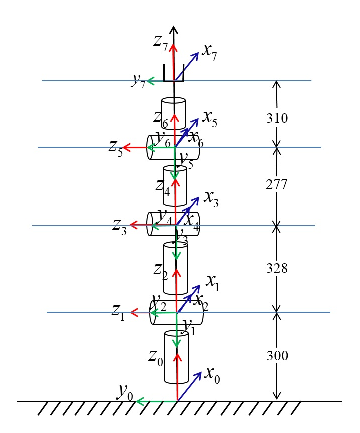
\includegraphics{robotaxis.eps}
}}
      \caption{Robot axis coordinates, obeying D-H parameter method, numbers in the graph is in milimeter.}
      \label{figurelabel}
   \end{figure}
   
As a result of this axis coordinates, we get the DH parameters as follow (show in TABLE I) :

\begin{table}[h]
\caption{$DH\ Parameters\ of\ robot.\ (\theta: joint\ angle;\ d: connecting\ rod\ skew;\ a: connecting\ rod;\ \alpha: tortuosity\ angle\ of\ connecting\ rod.)$}
\label{table1}
\begin{center}
\begin{tabular}{c|ccccc}
\hline
Joint Number & $\theta_i$ & $d_i$(mm) & $a_i$(mm) & ${\alpha_i}$(\degree) & area of $\theta_i$(\degree) \\
\hline
1 & $q_1$ & 300 & 0 & -90 & -180$\sim$180\\
2 & $q_2$ & 0 & 0 & 90 & -90$\sim$90 \\
3 & $q_3$ & 328 & 0 & -90 & -180$\sim$180\\
4 & $q_4$ & 0 & 0 & 90 & -120$\sim$120\\
5 & $q_5$ & 277 & 0 & -90 & -180$\sim$180\\
6 & $q_6$ & 0 & 0 & 90 & -120$\sim$120\\
7 & $q_7$ & 310 & 0 & 0 & -180$\sim$180\\
\hline
\end{tabular}
\end{center}
\end{table}

All our later works are based on table 1 and fig.1,  including experiments and simulation. As we can see in fig.1, the joint angles from $q_1$ to $q_7$ are the free variables and the others are fixed within our experiments. So when we write rotation and translation matrix in homogeneous way, which is a 4$\times$4 matrix, we can get the transformation equation from current coordinate ($x_i$, $y_i$, $z_i$) to the next coordinate ($x_{i+1}$, $y_{i+1}$, $z_{i+1}$) as (1):

$$
\begin{array}{cc}
^{i-1}T_{i} = A_{i} = &Rot(z, \theta_{i})\cdot \ Trans(0, 0, d_{i}) \ \cdot \\\ &Trans(a_{i}, 0, 0) \ \cdot \ Rot(x, \alpha_{i}). \\\ 
\end{array}
  \eqno({1})
$$ 

Among (1), Rot(z, $\theta$) means homogeneous transformation matrix when rotatting the current coordinate $\theta$ degree around z-axis, and Trans(x, y, z) means homogeneous transformation matrix when transform the current cordiante with the vector $\vec{v} = (x, y, z)$. 

Then, we can get the transformation matrix from base coordinate ($x_0$, $y_0$, $z_0$) to the end manipulator coordinate ($x_7$, $y_7$, $z_7$) as (2):

$$
M \ = \ ^{0}T_{1} \ ^{1}T_{2} \ldots ^{6}T_{7} \eqno({2})
$$

\subsection{Status Space \& Configuration Space}

Status Space is expressed with 7 parameters from $q_1$ to $q_7$, with the expression like (3):

$$
S \ = \ (q_{1}, q_{2}, \ ...  \ , q_{7}) \eqno({3})
$$

As for the configuration space, i.e., pose space, we use Euler angles that obeys Euler Z-X-Z transformation rules to express the azimuth angles, which displays like $\gamma = (\psi, \theta, \phi)$. Position writes like $P=(x,y,z)$. Get the position and Euler angles together, we define the expression of pose like (4):

$$
X = (P,\gamma) = (x,y,z,\psi,\theta,\phi) \eqno({4})
$$

See that S is expressed with 7 free variables while X with 6,  which tells the redundancy of our system, on which our work is based. 

\subsection{Forward Kinematics \& Jacobian Matrix}

As we can see in (2) \& (3),  M is decided by the current state S,  thus the current pose X is also decided. When we transform X into homogeneous matrix defined as $H(X)$ and write M as $M(S)$ (means M is decided by S), we get the connection between S and X:

$$
H(X) = M(S) \eqno({5})
$$

That is what our forward kinematics based on. Knowing the current S, we can get $M(S)$ from (2), then use (5) to get X. The detail operation from H(X) to X will not be discussed here, which can be easily found in primary textbook of robot kinematics. Combining the process of  turning $H(X)$ to X in M, we can finally get forward kinematics as below:

$$
X = M(S) \eqno({6})
$$ 

The letter M in (6) is not the same meaning with (2) \& (5), which combines the process from $H(X)$ to X. We can see M here in (6) as just a function with independent variables S and dependent variables X.

\subsection{Inverse Kinematics \& the Extend Inverse Jocobian Matrix}

Inverse kinematics comes with the question: how could we get S when we know X? Since the system is reduntant, there may not be one answer for S.  There are methods from X to S directly using fixed angle method, but in this paper we do inverse kinematics with the help of Jacobian matrix instead. 

Looking back at (6), we write M in partial form: 

$$
X = 
\left[
\begin{array}{c}
X_{1} \\
X_{2} \\
X_{3} \\
X_{4} \\
X_{5} \\
X_{6} \\
\end{array}
\right]
=
\left[
\begin{array}{c}
M_{1}(q_{1}, q_{2}, \ldots , q_{7}) \\
M_{2}(q_{1}, q_{2}, \ldots , q_{7}) \\
M_{3}(q_{1}, q_{2}, \ldots , q_{7}) \\
M_{4}(q_{1}, q_{2}, \ldots , q_{7}) \\
M_{5}(q_{1}, q_{2}, \ldots , q_{7}) \\
M_{6}(q_{1}, q_{2}, \ldots , q_{7}) \\
\end{array}
\right]
\eqno({7})
$$

The Jacobian Matrix is defined as (8):

$$
\begin{array}{ll}
J & = (\frac{\partial M}{\partial q_{1}},\frac{\partial M}{\partial q_{2}}, \ \ldots  \ , \frac{\partial M}{\partial q_{7}})   \\
\\
& = 
\left[
\begin{array}{cccc}
\frac{\partial M_{1}}{\partial q_{1}}, & \frac{\partial M_{1}}{\partial q_{2}}, & \ldots & \frac{\partial M_{1}}{\partial q_{7}} \\
\frac{\partial M_{2}}{\partial q_{1}}, & \frac{\partial M_{2}}{\partial q_{2}}, & \ldots & \frac{\partial M_{2}}{\partial q_{7}} \\
\vdots & \vdots & \ddots & \vdots \\
\frac{\partial M_{6}}{\partial q_{1}}, & \frac{\partial M_{6}}{\partial q_{2}}, & \ldots & \frac{\partial M_{6}}{\partial q_{7}} \\
\end{array}
\right]
\\
\end{array}
\eqno({8}) 
$$

In our expremental environment, the Jacobian matrix should be a 6$\times$7 matrix for 6 pose variables and 7 joint angle variables, but it should be reminded that this is not the same with all redundant manipulators. Then we get the relation between X and S in differential way:

$$
\dot{X} = J\dot{S} = J(\dot{q_{1}}, \dot{q_{2}}, \ldots, \dot{q_{7}}) \eqno({9})
$$

We can't use the direct inverse matrix of J to do inverse kinematics, but can do it with the generalized inverse matrix of J ($J^{+}$) defined like this:

$$
J^{+} = J^{T}(JJ^{T})^{-1} \eqno({10})
$$

In generalized form, we have:

$$
\dot{S} = J^{+}\dot{X} \eqno({11})
$$
$$
S - S_{0} = \Delta S = J^{+}\Delta X = J^{+} (X - X_{0}) \eqno({12})
$$

In this way, when knowing the initial pose $X_{0}$, very near pose X, and the initial $S_{0}$, we can compute the status S relative to X according to (11)(12), which is our inverse kinematics mainly based on, both for MLG and Newton-Raphson method we will introduce later.

\section{RRT with extended steps}

Since we use modified RRT to do obstacle-avoiding path planning, we can have a look at the initial RRT method to better understand the results. In this chapter, we study RRT and its relevant algorithms in a more detail way.

\subsection{Pre-definition before RRT}

We define the relevant collections and functions of RRT below before looking at its pseudocode. Reminded the basic problem RRT do with first:  how can we run the manipulator from the initial position (knowing $S_{0}$ \& $X_{0}$) to the goal position (only knowing pose of end position, taken down as $X_{g}$), without collision with the obstacles in the space? The following collections are defined to express RRT in convenience:

\begin{itemize}

\item $A_{0}$: the whole pose space which can be reached by robot manipulator in configuration space.

\item $A_{free}$: free space belong to $A_{0}$, i.e., $A_{free} \in A_{0}$, and there is no obstacle in $A_{free}$. 

\item $A_{obs}$: space of obstacle, i.e., $A_{obs} = A_{0}  \backslash A_{free}$.

\item $B_{0}, B_{free}, B{obs}$: these are the corresponding collections with A, but in the status space. The subscript takes the same meaning as in A.

\end{itemize}

Below define the main functions used in RRT. Before we focus on these functions, we should remind that RRT method will build a tree when it runs, we called it RRT tree, writen as tree $T$, with the initial point $X_{0}$ for pose and  $S_{0}$ for status as the first tree point. We note that: $T = (V, E)$, while V stands for all points and E is the relation between these points (father point and its child). Note that $T$ is a tree, so each $||E||=||V||-1$. Then, we have a look at the basic functions which RRT method use.

\begin{itemize}

\item sample:  generates a random point $X_{ram}$ in pose format within $A_{free}$.

\item distance:  compute the distance of two points in $A_{0}$. Within our program, this distance is defined near to the Euclid distance, see it in (13).

\item nearest\_neighbor: given the point X, this function returns the nearest point $X_{near}$ to X in tree $T$.

\item steer: given the random point $X_{ram}$ and $X_{near}$, this function returns a new point $X_{new}$ in $A_{free}$, which is nearer to $X_{ram}$ than $X_{near}$.

\item collisionTest: given point $X$, return 1 for obstacle free and 0 for obstacle collision. 

\end{itemize}

\subsection{RRT and its relative functions}

Then we can have a look at the basic algorithm of RRT. We write it in pseudocode show in Fig. 2:

\begin{figure}[thpb]
      \centering
      \framebox{
      \parbox{3in}
      {
      $
      RRT (S_{0}, A_{0})\\
      1.\ V \leftarrow \{S_{0}\}; E \leftarrow \o; i \leftarrow 0;\\
      2.\ while\ i < N\ do \\
      3.\ \{ \\
      4.\qquad T \leftarrow (V,\ E); \\
      5.\qquad X_{rand} \leftarrow sample(i); i \leftarrow i+1; \\
      6.\qquad T \leftarrow extend(T, X_{rand});\\
      7.\ \} \\
      $
      \\
      $
      extend(T, X_{rand}) \\
      1.\ X_{near}=  nearest\_neighbor(T, X_{rand});\\
      2.\ X_{new} = steer(X_{near}, X_{rand});\\
      3.\ if\ X_{new}\ and\ collisionTest(X_{new})\\\
      4.\qquad V \leftarrow V \cup \{X_{new}\};\\
      5.\qquad E \leftarrow E \cup \{(X_{near}, X_{new})\};\\
      5.\qquad return\ success;\\
      6.\ else\\
      7.\qquad return\ fail;
      $
	 }
}
      \caption{pseudocode of RRT algorithm.}
      \label{figurelabe2}
\end{figure}
 
 Though simple as it is, RRT method works well with obstacle-avoiding task. Here, we focus on the detail equation of the basic functions specially, for they will be related later in this paper. As defined before, we use Euclid distance but make a little change, named `rrtDistance', which is defined with (13):
 

 $$
 \begin{array}{ll}
 &rrtDistance(X_{1},X_{2})=\alpha ||P_{1}-P_{2}|| + \\
& \qquad\qquad (1-\alpha) ||\gamma_{1}-\gamma_{2}||, \ 0 < \alpha < 1. 
\end{array}
\eqno(13)
 $$

   
 Since we concentrate more on the accuracy of position, we mainly choose $\alpha > 0.5$, like $\alpha = 0.8$, which is use in our program.  The sample function generates a point in $A_{0}$, we use $X_{min}$ and $X_{max}$ to limit area of $A_{0}$. Then the random point $X_{ram}$ that sample function produces will be like (14):
 
 $$
 X_{ram} = X_{min} + t \times (X_{max}-X_{min}), 0<t<1;
 \eqno({14})
 $$
 
When t is randomly produced in interval (0, 1), sample method would produce all the points of $A_{0}$. For steer function, a new point $X_{new}$ will be produce depending on $X_{near}$ and $X_{ram}$,  which works like (15):
 
 $$
 \begin{array}{rr}
 X_{new} = X_{near} + s(X_{ram}-X_{near})/||X_{ram}-&\\
 X_{near}||,\ 0<s<||X_{ram}-X_{near}||.&
 \end{array}
 \eqno(15)
 $$
 
 We call $s$ in (15) the step-length. In RRT algorithm, each time when steer function runs, the RRT tree $T$ will attend to explore forward $s$ distance in $A_{0}$. Because $X_{rand}$ will be anywhere in the whole space, it is easy to infer that the direction tree $T$ extends is all-dimension, i.e., no certain direction, but different directions with different times, reminded this in mind cause we will discuss it later.
 
\subsection{Modified RRT algorithm}

Though RRT can explore the whole space $A_{0}$ to get a obstacle-free path to reach the goal point, it still has some shortage when it actually runs. Since RRT extends only one step (with step-length $s$) further each time, it seems slow sometimes when $A_{0}$ is big enough to explore. On the other point, RRT tree are built beginning with the initial point, leaving out the goal point in the tree-built process. Still, there are other insufficients with RRT, which results in many modified RRT methods. Here, we present bi-RRT as an example. More detail bi-RRT algorithm pseudocode can be seen in [11]. We just take it in brief here.

As the shortages we tell above, bi-RRT solves it by extending more steps until in collision with obstacle or reach the random point $X_{ram}$.  And bi-RRT maintains two trees in its memory, one starting extend function from the initial point and the other from the goal point. The two trees extend to each other exchangely every time, when `extend' method runs until they meet in the space, which is the reason the name `bi-RRT' comes from. With such modification, bi-RRT takes in account of both the intial point and goal point together with a faster extending speed. 

In our exprement, we just take the thought of more steps extending strategy into our program. Our multi-extend algorithm is written like Fig. 3:

\begin{figure}[thpb]
      \centering
      \framebox{
      \parbox{3in}
      {
      $
      multi\_extend(T, X_{rand})\\
      1.\ [X_{new}, result] = extend(T, X_{rand});\\
      2.\ if\ result = fail\ or\ collisionTest(X_{new}) = 0\\
      3.\qquad return\ fail;\\
      4.\ while\ result = success \\
      5.\ \{ \\
      6.\qquad [X_{new}, result] = extend(X_{new}, X_{rand});\\
      \begin{aligned}
      7.\qquad if\ collision&Test(X_{new}) = 0\ or\ \\ &surpass(X_{new}, X_{rand})\\
      \end{aligned} \\
      8.\qquad \qquad break; \\
      9.\ \} \\
      10.\ return\ success.
      $
	 }
}
      \caption{multi-step extend pseudocode}
      \label{figurelabe3}
\end{figure}

The function `$surpass(X_{new},X_{rand})$' detect that if $X_{new}$ is near enough to $X_{rand}$. The `true' return for this function means the two points are close enough, then `multi\_extend' method will be stopped, and the `false' return will continue the extending process.  With these change, if the extending direction is correct, i.e., closer to goal point, we could get faster to the goal point, but simutaneously, we would also extend further to a bad direction, which would take up more time if this situation happens frequently. We solve this problem with RRT-GD (RRT with goal-directionality), which will be related in the later paragraph. But within our process now, we have two extend strategies: `extend' and `multi-extend'. And we can think of the inverse kinematics optimization after finishing RRT method.

\section{Inverse Kinematics with Newton-Raphson method}

We have related some inverse kinematics method before, e.g., GP (gradient projection method), WLN (weighted least norm method), MLG (most likely gradient)[3]. Within our program, we take Newton-Raphson method into account, for its high accuracy and speed. 

\subsection{Newton-Raphson method}

Let's come back to our inverse kinematics problem: we know $S_{0}$ (and so $X_{0}$ can be compute) and $X_{g}$, how could we compute $S_{g}$? In Newton-Raphson method, which is an iteration method, each time we just go straight from the current point to goal point. We can see in the iteration equation in (16):

$$
S_{n+1} = S_{n} + J^{+} \times minus(X_{g}, X_{n}).
\eqno(16)
$$ 

The current status and pose are written as $S_{n}$ and $X_{n}$, and $J^{+}$ is also relative to the current point, which can be compute in (10). Then when $X_{n}$ is close enough to $X_{g}$, we get the answer $S_{n+1}$ as result $S_{g}$. Note that though the function name called `minus', it didn't just do simple minus operation as $X_{g} - X_{n}$, because the azimuth doesn't supplement the minus operation. We should use the Rotate-By-1-Axis method to get the corret answer, since the combination of any fix-axis rotations of rigid body can be seen as one-time fix-axis.

After this work, we take down the Newton-Raphson method as Fig. 4.

\begin{figure}[thpb]
      \centering
      \framebox{
      \parbox{3in}
      {
      $
      Newton\_Raphson(S_{0}, X_{g})\\
      1.\ compute\ X_{0}\ and\ J^{+}; i = 0; times = 0;\\
      2.\ while\ \epsilon < rrtDistance(X_{i}, X_{g})\ and\ times < N\\
      3.\ \{ \\
      4.\qquad S_{i+1} = S_{i} + J^{+}\times minus(X_{g}, X_{i});\\
      5.\qquad i = i + 1;times = times + 1;\\
      6.\qquad compute\ X_{i}\ and\ J^{+};\\
      7.\ \}
      $
	 }
}
      \caption{multi-step extend pseudocode}
      \label{figurelabe4}
\end{figure}

On Fig.4, the 1st and 6th line use (6) and (10) to compute relative parameters. Here we use N (we set it to 10 in program) to limit the iteration times, for the fact that Newton-Raphson method would always get the correct answer in less than 10 iteration times with accuracy of micrometer, otherwise it would fail with bias greater than $\epsilon$ (1 micrometer), i.e., more iteration times have no use cause it can't improve the accuracy further more.  

\subsection{Comparation with MLG}

At the beginning, we have complemented the MLG method before using Newton-Raphson method for inverse kinematics. Here, we introduce MLG method and compare it with Newton-Raphson method, to see some great properties of Newton-Raphson algorithm.

MLG method is also a iteration method, using the gradient of current point as the iteration direction, the detail of which can be seen in [3]. We just make comparation between MLG and Newton-Raphson method.

\begin{table*}[h]
\caption{$Comparation\ between\ RRT\ and\ $ Newton-Raphson $ method.\ S_{0} = [0.7854;0.5236;0;0.5236;0;0.5236;0](rad);\ X_{0}=[0.5045;0.5045;0.7223;2.3562;1.5708;-1.5708];\ dist = rrtDistance(X_{0}, X_{g}), all\ their\ units\ are\ meters(m). `\surd'\ means\ successful.\ `\times'\ means\ result\ failed,\ i.e.,\ bias\ (accuracy)\ comes\ out\ more\ than\ 0.1m.$}
\label{table2}
\begin{center}
\begin{tabular}{c|c|c|c|c|c|c}
\hline
No. & task(m) & Method & iteration times & time spent($10^{-3}s$) & accuracy(m) & result \\
\hline
\multirow{4}{*}{1}  &
\multirow{4}{*}{
$
\begin{array}{l}
X_{g} = 
\left[
\begin{array}{c}
0.50; 
0.45;
0.72;
2.35;
1.57;
-1.57
\end{array}
\right] \\ \\
dist = 0.045.
\end{array}
$}
  & N-R & 5 & $6.15$ & $1.28\times 10^{-9}$ & $\surd$ \\
\cline{3-7}
  &    &         & 5 & $5.70$ & $6.50\times10^{-3}$ & $\surd$ \\ \cline{4-7}
   &    & MLG & 10 & $6.52$ & $2.64\times10^{-3}$ & $\surd$ \\ \cline{4-7}
   &    &         & 20 & $11.76$ & $1.25\times10^{-3}$ & $\surd$ \\ 
\hline
\multirow{4}{*}{2} & 
\multirow{4}{*}{
$
\begin{array}{l}
X_{g} = 
\left[
\begin{array}{c}
0.5;
0.48;
0.72;
2.35;
1.55;
-1.55
\end{array}
\right] \\ \\
dist = 0.025.
\end{array}
$
}
& N-R & 4 & 2.38 & $2.34\times10^{-7}$ & $\surd$ \\
\cline{3-7}
 &     &         & 5 & 3.95 & $9.74\times10^{-2}$ & $\surd$\\
\cline{4-7}
 &     &  MLG &10& 6.60 & $9.56\times10^{-2}$ & $\surd$\\
 \cline{4-7}
 &     &         &20& 12.77& $9.39\times10^{-2}$ & $\surd$\\
\hline
\multirow{4}{*}{3}
&
\multirow{4}{*}{
$
\begin{array}{l}
X_{g} = 
\left[
\begin{array}{c}
0.44;
0.44;
0.68;
2.30;
1.57;
-1.57
\end{array}
\right] \\ \\
dist = 0.092.
\end{array}
$
}
& N-R & 7 &3.87 & $5.87\times10^{-8}$ & $\surd$ \\
\cline{3-7}
 &    &        & 5 & 3.94 & $1.65\times10^{-2}$ & $\surd$ \\
\cline{4-7}
 &    & MLG &10& 6.64 & $1.73\times10^{-2}$ & $\surd$ \\
 \cline{4-7}
 &    &         &20& 12.20& $1.78\times10^{-2}$ & $\surd$ \\
 \hline
\multirow{4}{*}{4}
&
\multirow{4}{*}{
$
\begin{array}{l}
X_{g} = 
\left[
\begin{array}{c}
0.45;
0.55;
0.60;
2.00;
1.57;
-1.57
\end{array}
\right] \\ \\
dist = 0.184.
\end{array}
$
}
& N-R & 9 &5.70 & $5.53\times10^{-10}$ & $\surd$ \\
\cline{3-7}
 &    &        & 5 & 4.46 & $1.37\times10^{-1}$ & $\times$ \\
\cline{4-7}
 &    &  MLG &10& 7.31 & $1.22\times10^{-1}$ & $\times$ \\
 \cline{4-7}
 &    &         &20& 11.65& $1.12\times10^{-1}$ & $\times$ \\
 \hline 
\end{tabular}
\end{center}
\end{table*}

We do comparation between these two methods using 4 groups of experiments. These tests start with the same initial point $q_0$, and so the same with $X_0$, and go to different end point appointed by $X_{g}$. Note that the iteration times of MLG method can be a input variable which can be assigned before MLG algorithm runs. So we take 5, 10, and 20 iteration times as examples. As TABLE II shows, in these groups of exprements, we make sense that:

\begin{itemize}

\item  The time spent by Newton-Rapshon method is almost the same with 5-iteration-times MLG method doing the same task, sometimes even less than it.
\item  Newton-Raphson method uses less than 10 iteration times ending up with bias no more than $10^{-6}m$, but MLG method, no matter using 5, 10, or 20 iteration times, always ending up with deviation error higher than $10^{-3}m$, spending time in the same order of Newton-Raphson method.  
\item Newton-Raphson method adapts to a wider range of `dist' change, i.e., it is suitified to more tasks when doing inverse kinematics. When `dist' becomes bigger, Newton-Raphson works better than MLG method, that can be find in group 4, with Newton-Raphson method successful and MLG failed. Here, we limit the result bias to $0.1m$, i.e., when the accuracy is bigger than this number, we think it failed. 
\item When Newton-Raphson method fails in doing inverse kinematics, MLG method may always can't work well, because they both use the gradient of current point. Minded that whether the result fail or success doesn't depend on `dist' parameter, it is decided by many reasons. Sometimes a small `dist' even like $0.02m$ may also result in failed both for Newton-Raphson method and MLG method.

\end{itemize}

One point which should be reminded is that we implement MLG method according to [3]. There exists some limitaion conditions with the end trajectory, e.g., the velocity of end manipulator can't be 0, which is set to faster than $0.05m/s$ in our program. So more iteration times may not makes the more accuracy in MLG method. But the conclusion that MLG method always ends up with accuracy of $10^{-3}m\sim10^{-2}m$ when it successes is right, which has been tested by many times of experiments. 

\section{Quintic Polynomial with path smoothing}

There comes another question after doing Newton-Raphson method: knowing $S_{0}$ and $S_{g}$, how could we move the manipulor? The most direct answer might be simply adapt the joint angle to $S_{g}$, however, we can't know the trajectory of the end manipulator in this way, and it might be also not the shortest distance in the thought of end manipulator. Thus, we need to smooth the path from $S_{0}$ to $S_{g}$. 

MLG method can do the path smoothing in its iteration, i.e., when finishing compute $S_{g}$, it also finishes planning the path from $S_{0}$ to $S_{g}$, with a designing trajectory (usually a straight line) of the end manipulator. But the same thing can't apply to Newton-Raphson, for its variant iteration times and variant distance between adjacent points within one iteration. So we need to do path planning separately. The quintic polynomial thus has been used in our program, the principle of which can be seen in [9]. We just use its conclusion. Supposed we know $S_{0}$, $S_{g}$, and their distance ($rrtDistance(S_{0}, S_{g}) =s$, see in (15)) fixed, we need to plan the medium path in 1 second (of course it can be changed by timing a factor). Then in quintic polynomial method, we plan the path as in (17):

$$
\begin{array}{c}
S(t) = a_{5}t^5+a_{4}t^4+a_{3}t^3+a_{2}t^2+a_{1}t+a_{0};\\
with:
\left \{
\begin{array}{ll}
a_{5} = &6(S_{g}-S_{0});\\
a_{4} = &-15(S_{g}-S_{0});\\
a_{3} = &10(S_{g}-S_{0});\\
a_{2} = &0;\\
a_{1} = &0;\\
a_{0} = &S_{0};\\
\end{array}
\right.
\end{array}
\eqno(17)
$$

We can see in (17) of the kinematics properties of its planning path. When $t = 0s$, $S(t)$ equals to $S_{0}$, that is the initial point;  and when $t = 1s$, $S(t)$ equals to $S_{g}$, that is the goal point. And we can also compute the speed at each time in the path, just by doing differential operation. What we can deduce from (17) is that the speed of end manipulator when in initial point or goal point is 0. We could also change the coefficients from $a_{0}$ to $a_{5}$ according to [9] to fit different uses. These method works well on our 7-arm robot manipulator when doing exprements.

\section{RRT-GD: turn RRT to be goal-directionality}

When finishing the work above, we can already finishing any work in the work space in theory. But just as the problem we have mentioned before, both RRT and its modified method have the great opportunity to explore unuseful space which we don't need in our daily task, i.e., it lacks goal-directionality. In order to solve this problem, taking the normal task in our experiment circumstance into account, we turn our sights to the `sample' function in RRT. Simple to find that if we just don't use a whole space `sample' method, but limit it to a useful space, we can decide the extending direction of RRT tree $T$, that is the kernel principle within our modified RRT method called RRT-GD.

Originally, `sample' method is random in the whole work space, thus its extend direction is all-around. The sketch map can be seen in Fig. 5. When we use a space containning the goal point $X_{g}$, called sample space $A_{sam}$, which can simply be a sphere with $X_{g}$ centering (of course other shapes also works, e.g., cuboid), the extending direction can be limit to goal-direction, as Fig.5 shows. We can deduce from the sketch map that, if the initial point is contained in sample space, i.e., $X_{0}\in A_{sam}$, then the extending direction could also be all-around just as usual RRT does, but since the times random point is produced in the contrary of goal-direction become less, the goal-direction extending could also become more than usual RRT method. In our experiments, we choose sample space without the initial point, to see the goal-direction property of RRT-GD more clear.

We implement our `sample' method with sample space in sphere shape of radius set to $0.5m$. We can see the comparation between RRT and RRT-GD within iteration times and time property in TABLE III.

\begin{figure*}[thpb]
      \centering
      \framebox{
      \parbox{7in}{
      \subfigure[Extend direction of RRT: all-direction.]
      {
      \label{Subfig.1}
      \includegraphics[width=8cm, height=4.2cm]{ext2whole.eps}	
      }
      \subfigure[Extend direction of RRT-GD: goal-direction.]
      {
      \label{Subfig.2}
      \includegraphics[width=8cm, height=4.2cm]{ext2sample.eps}	
      }
      }
      }
      \caption{Extend direction of RRT and RRT-GD. Pink cuboid is for the whole working space. Blue sphere is for sample space. }
      \label{figurelabe5}
\end{figure*}

\begin{table*}[h]
\caption{$Comparation\ between\ $RRT$\ and\ $RRT-GD$\ method.\ S_{0} = [-0.2618;-0.2618;0;-1.3090;0;-1.3962;0](rad);\ X_{0}=[0.4011;0.1075;0.3115;-1.8326;2.9671;1.5708];\ dist = rrtDistance(X_{0}, X_{g}), all\ their\ units\ are\ meters(m). `\times'\ means\ result\ failed.$}
\label{table3}
\begin{center}
\begin{tabular}{c|c|c|c|c|c}
\hline
No. & task(m) & Method & extending times & failed extending times &time spent($s$) \\
\hline
\multirow{2}{*}{1}  &
\multirow{2}{*}{
$
\begin{array}{l}
X_{g} = 
\left[
\begin{array}{c}
0.42; 
-0.22;
0.22;
-1.83;
2.97;
-1.57
\end{array}
\right] \\
dist = 0.7108.
\end{array}
$}
  & RRT & 808 & 8401 & 108.20 \\
\cline{3-6}
  &    &  RRT-GD & 9 & 27 & 0.44 \\
\hline
\multirow{2}{*}{2} & 
\multirow{2}{*}{
$
\begin{array}{l}
X_{g} = 
\left[
\begin{array}{c}
0.42;
0.22;
0.22;
-1.83;
2.80;
-1.50
\end{array}
\right] \\
dist = 0.6668.
\end{array}
$
}
& RRT & 506 & 4250 & 47.39 \\
\cline{3-6}
 &     &  RRT-GD & 3 & 1 & 0.16 \\
\hline
\multirow{2}{*}{3}
&
\multirow{2}{*}{
$
\begin{array}{l}
X_{g} = 
\left[
\begin{array}{c}
0.51;
0.12;
0.22;
-1.73;
2.90;
-1.57
\end{array}
\right] \\
dist = 0.7326;
\end{array}
$
}
& RRT & \multicolumn{3}{c}{$\times$} \\
\cline{3-6}
 &    & RRT-GD & 4 & 6 & 0.219 \\
 \hline
\end{tabular}
\end{center}
\end{table*}

\begin{figure*}[thpb]
      \centering
      \framebox{
      \parbox{7in}{
      \subfigure[RRT in Group No.1 of table 3]
      {
      \label{Subfig.1}
      \includegraphics[width=8cm, height=4.2cm]{RRT1.eps}	
      }
      \subfigure[RRT-GD in Group No.1 of table 3]
      {
      \label{Subfig.2}
      \includegraphics[width=8cm, height=4.2cm]{RRTGDNICE.eps}	
      }
      }
      }
      
      \framebox{
      \parbox{7in}{
      \subfigure[RRT in Group No.2 of table 3]
      {
      \label{Subfig.3}
      \includegraphics[width=8cm, height=4.2cm]{RRT2.eps}
      }
      \subfigure[RRT-GD in Group No.1 of table 3]
      {
      \label{Subfig.4}
      \includegraphics[width=8cm, height=4.2cm]{RRTGD2.eps}	
      }
      }
      }
      \caption{Result comparation between RRT and RRT-GD. The blue sphere is the sample method sphere we use with goal point centering in red. The range of pink cuboid is our whole work space. The yellow sphere or cuboid is obstacle in the free space. The crayon line is the planning path starting from initial point to goal point. }
      \label{figurelabe6}
\end{figure*}

We take the same initial point as $S_{0}$ in TABLE III, and let the end manipulator go to different goal points. The `extending times' in table 3 is the total times of successful extending when finding the exact path to goal point, and `failed extending times' means the total failed times when doing extending. The altogether iteration is their sum. One point which should be reminded is that the data in TABLE III is only one successful result among many tests, which is the mid-value within these tests. From Table III and Fig. 6, we can learn that:

\begin{itemize}

\item RRT-GD uses much less time and iteration times compared to RRT when doing the same work. As we can see, RRT-GD attends to be 100 times faster, speeding up the algorithm remarkably.
\item RRT-GD can almost be realtime path planning in these tasks, with planning time less than 0.5$s$, which is a great improment when comparing to the traditional RRT method.
\item RRT-GD can do the task that RRT can't, as in task 3 of TABLE III. Here, we set the iteration times limitation to 10000,  surpassing which we think the algorithm failed. In task 3, we do RRT method for 10 times but none of them succeed, while RRT-GD could always succeed.
\item Within our experiments, RRT-GD could succeed as long as RRT method succeed, i.e., the correctness of RRT-GD can be assured. This is because there are usually not so many obstacles in the working space, and each obstacle is usually small enough (no more than 0.1$s$ in radius), while the radius of sample space is set to 0.5$m$, that is big enough to do common works with obstacle-avoiding.
\item Since RRT-GD uses less iteration times, so the planning path gived by RRT-GD seems to be more directly, i.e., less zig-zag on the path, which can be seen in Fig. 6.

\end{itemize}

Note that we return the program immediately if it finds the planning path from initial point to goal point when doing the tasks in TABLE III Of course. Of course, we could also set iteration times to a fix number, then use RRT-GD or RRT method to get multiple paths and get the best one as output. When doing these way, says iteration times limitation to 10000, RRT-GD can always get more paths out than RRT method.

One more to say, we can think of the two peaks of RRT-GD. One situation is when sample space fills up the whole working space, i.e., $A_{sam} = A_{0}$. At this time, RRT-GD algorithm attends to be RRT method, i.e., they are the same when running. Another situation is that when sample space shrinks to only one point, i.e., $A_{sam} = \{X_{goal}\}$, then the problem becomes a straight line path planning from the initial point to goal point. In fact, since we can't give the whole space an accuracy limitation, RRT method itself thus can't ensure to give a path even the path truly exists, i.e., RRT isn't even correct in theory on the account of actual use in this way. So RRT-GD is an important ideology which proves to be more pratical, press closer to the real circumstance and daily common tasks. 



\section{CONCLUSIONS}

In this paer, we introduce a new method in obstacle-avoiding path planning, with modified RRT method doing obstacle-avoiding, Newton-Raphson doing inverse kinematics, and quintic polynomial doing path smoothing. After that, we find the less goal-direction with RRT and its modified algorithms, so we implement RRT-GD to solve this problem. With RRT-GD, we can accomplish daily works faster and more efficient, usually 10$\sim$100 times faster than the usual RRT method because of its goal-directionality property. Note that when the sample space of RRT-GD is not full of the whole working space, RRT-GD may not give a right planning path as RRT in theory, i.e., it is not a usual method. However, RRT-GD works well in practice, as we can see in TABLE III and Fig. 6, for that in our common working space, there are usually not so many obstacles and the size of each obstacle are usually small enough for RRT-GD to work on well.

\addtolength{\textheight}{-12cm}   % This command serves to balance the column lengths
                                  % on the last page of the document manually. It shortens
                                  % the textheight of the last page by a suitable amount.
                                  % This command does not take effect until the next page
                                  % so it should come on the page before the last. Make
                                  % sure that you do not shorten the textheight too much.

%%%%%%%%%%%%%%%%%%%%%%%%%%%%%%%%%%%%%%%%%%%%%%%%%%%%%%%%%%%%%%%%%%%%%%%%%%%%%%%%



%%%%%%%%%%%%%%%%%%%%%%%%%%%%%%%%%%%%%%%%%%%%%%%%%%%%%%%%%%%%%%%%%%%%%%%%%%%%%%%%



%%%%%%%%%%%%%%%%%%%%%%%%%%%%%%%%%%%%%%%%%%%%%%%%%%%%%%%%%%%%%%%%%%%%%%%%%%%%%%%%



%%%%%%%%%%%%%%%%%%%%%%%%%%%%%%%%%%%%%%%%%%%%%%%%%%%%%%%%%%%%%%%%%%%%%%%%%%%%%%%%



\begin{thebibliography}{99}

\bibitem{c1} A Methodology for Intelligent Path Planning, Suman Chakravorty, John L. Junkins. Department of Aerospace Engineering, Texas A\&M University Young, College Station.
\bibitem{c2} Kinect-based Service Robot for Desktop Cleaning, Zheng Han, Meng Gao, ShiJiaZhuang Tiedao University.
\bibitem{c3} Planning Method Considering the kinetic characteristics of the end effector of a redundant manipulator, Wenbing Huang, Fuchun Sun, Huaping Liu, Qinghua Daxue Xuebao/journal of Tsinghua University, 2014,54(12):1544-1548.
\bibitem{c4} Incremental kinesthetic teaching of motion primitives using the motion refinement tube, Dongheui Lee, Chritian Ott, Autonomous Robots, 2011, 31(2-3):115-131.
\bibitem{c5} New Heuristic Algorithms for Efficient Hierarchical Path Planning,  David Zhu and Jean-Claude Latombe, IEEE Transactions on Robotics \& Automation, 1991.7(1):9-20.
\bibitem{c6} A Subdivision Algorithm in Configuration for Findpath with Rotation, Rodney A. Brooks, Tomas Lozano-Perez, Systems Man \& Cybemetics IEEE Transactions on, 1985, SMC-15(2):244-233.
\bibitem{c7} Motion Planning and Skill Transfer of Anthropomorphic Arms Based on Movement Primitives,Xilun Ding, Cheng Fang, International Conference on Mechatronics \& Automation, 2012:303-310.
\bibitem{c8} Algorithm Based on Analytical Method and Genetic Algorithm for Inverse Kinematics of Redundant Manipulator, Yun Dong, Tao Yang, Wen Li, Computer Simulation, 2012.
\bibitem{c9} Trajectory Planning for a Robotic Ping-pong Player, Guowei Zhang, Bin Li, Huaibing Zhen, Haili Gong, Cong Wang, Chinese Journal of Scientific Instrument, Vol.32 No.6, Jun 2011.
\bibitem{c10} Virtual Reality in the Loop – Providing an Interface for an Intelligent Rule Learning and Planning System, Jurgen Rossmann, Christian Schlette, Nils Wantia, IEEE International Conference on Robotics \& Automation, 2013.
\bibitem{c11} Research on Kinematics and Obstacle Avoidance Path Planning for Redundant Manipulator, Yin Bin, Shi Shicai, Classified Index:TP242.2, U.D.C:681.5.






\end{thebibliography}




\end{document}
